\documentclass[11pt,letterpaper]{article}

% Packages
\usepackage[utf8]{inputenc}
\usepackage[T1]{fontenc}
\usepackage{amsmath,amssymb,amsthm}
\usepackage{algorithm}
\usepackage{algorithmic}
\usepackage{graphicx}
\usepackage{hyperref}
\usepackage{xcolor}
\usepackage{booktabs}
\usepackage{tikz}
\usetikzlibrary{shapes,arrows,positioning,calc}
\usepackage{listings}
\usepackage{caption}
\usepackage{subcaption}
\usepackage[margin=1in]{geometry}

% Theorem environments
\newtheorem{theorem}{Theorem}[section]
\newtheorem{lemma}[theorem]{Lemma}
\newtheorem{proposition}[theorem]{Proposition}
\newtheorem{corollary}[theorem]{Corollary}
\newtheorem{definition}{Definition}[section]
\newtheorem{example}{Example}[section]

% Custom commands
\newcommand{\Zoo}{\textsc{Zoo}}
\newcommand{\Zen}{\textsc{Zen}}
\newcommand{\DSO}{\textsc{dso}}
\newcommand{\FDSO}{\textsc{fdso}}
\newcommand{\LLM}{\textsc{llm}}
\newcommand{\FL}{\textsc{fl}}
\newcommand{\DP}{\textsc{dp}}

% Hyperref setup
\hypersetup{
    colorlinks=true,
    linkcolor=blue,
    citecolor=blue,
    urlcolor=blue
}

% Title and authors
\title{\textbf{Federated Decentralized Self-Optimization: Privacy-Preserving Distributed Learning for Language Models}\\
\large Version 1.0}

\author{
Zach Kelling\thanks{Corresponding author: zach@hanzo.ai}\\
\textit{Hanzo Industries Inc (Techstars '17)}\\
\textit{Lux Partners}\\
\textit{Zoo Labs Foundation}\\
\texttt{research@zoo.ngo}
}

\date{June 2024}

\begin{document}

\maketitle

\begin{abstract}
We present \textbf{Federated Decentralized Self-Optimization} (\FDSO{}), a framework for collaborative improvement of large language models without centralized data collection or gradient aggregation. \FDSO{} extends Decentralized Self-Optimization (\DSO{}) with privacy-preserving techniques that enable organizations to contribute to shared model improvement while keeping their data, interactions, and learned experiences strictly local. Our approach combines three innovations: (1) \textbf{Semantic Differential Privacy}---adding calibrated noise to experience embeddings rather than raw gradients, preserving retrieval utility while guaranteeing $(\epsilon, \delta)$-differential privacy, (2) \textbf{Byzantine-Robust Aggregation}---median-based experience selection that maintains system integrity with up to 30\% adversarial participants, and (3) \textbf{Homomorphic Experience Matching}---encrypted similarity computation enabling cross-organizational retrieval without revealing experience contents. We prove that \FDSO{} achieves equivalent model improvement to centralized training ($<2\%$ performance gap) while providing formal privacy guarantees. Experimental evaluation across 50 organizations with heterogeneous data distributions demonstrates 23\% capability improvement over isolated training, 89\% reduction in communication costs compared to federated gradient methods, and successful privacy preservation under realistic attack scenarios.

\textbf{Keywords}: federated learning, differential privacy, decentralized AI, self-optimization, privacy-preserving machine learning
\end{abstract}

\section{Introduction}

Large language models achieve remarkable capabilities through training on massive datasets. However, the most valuable data---enterprise documents, medical records, legal cases, financial transactions---remains siloed within organizations due to privacy, regulatory, and competitive concerns. This creates a fundamental tension: the data that could most improve AI capabilities is precisely the data that cannot be shared.

Federated Learning (\FL{}) addresses this by training models on distributed data without centralization. But \FL{} faces challenges with language models:

\begin{itemize}
    \item \textbf{Communication Cost}: Exchanging gradients for billion-parameter models requires terabytes of bandwidth per round.

    \item \textbf{Heterogeneity}: Organizations have wildly different data distributions, causing gradient conflicts.

    \item \textbf{Privacy Leakage}: Gradients can leak training data through inversion attacks.

    \item \textbf{Synchronization}: Coordinating training across organizations with different schedules is operationally complex.
\end{itemize}

\subsection{From Gradients to Experiences}

Decentralized Self-Optimization (\DSO{}) offers an alternative: instead of sharing gradients, share \emph{semantic experiences}---natural language descriptions of successful reasoning patterns. This has several advantages:

\begin{enumerate}
    \item \textbf{Efficiency}: Experiences are kilobytes vs. gigabytes for gradients
    \item \textbf{Interpretability}: Humans can audit shared experiences
    \item \textbf{Asynchrony}: Organizations contribute experiences on their own schedules
    \item \textbf{Heterogeneity}: Experiences from diverse domains enrich capabilities
\end{enumerate}

However, naive experience sharing still raises privacy concerns. An experience like ``When analyzing patient symptoms including [X, Y, Z], the diagnosis of [condition] was confirmed'' leaks sensitive medical information.

\subsection{Contributions}

This paper introduces \FDSO{}, extending \DSO{} with rigorous privacy guarantees:

\begin{enumerate}
    \item \textbf{Semantic Differential Privacy}: Privacy-preserving experience sharing with formal $(\epsilon, \delta)$ guarantees (Section~\ref{sec:privacy})

    \item \textbf{Byzantine-Robust Aggregation}: Secure experience selection tolerating adversarial participants (Section~\ref{sec:byzantine})

    \item \textbf{Homomorphic Experience Matching}: Encrypted retrieval enabling private cross-organizational search (Section~\ref{sec:homomorphic})

    \item \textbf{Formal Analysis}: Proofs of privacy preservation and convergence (Section~\ref{sec:analysis})

    \item \textbf{Comprehensive Evaluation}: Empirical validation across diverse organizations (Section~\ref{sec:evaluation})
\end{enumerate}

\section{Background}

\subsection{Decentralized Self-Optimization}

\DSO{} enables language models to improve through experience sharing:

\begin{definition}[\DSO{} Experience]
An experience $e = (c, r, q)$ consists of:
\begin{itemize}
    \item $c$: Context (problem specification)
    \item $r$: Reasoning trace (solution approach)
    \item $q$: Quality score (human or automated evaluation)
\end{itemize}
\end{definition}

Models retrieve relevant experiences during inference, using them as in-context examples to improve performance.

\subsection{Differential Privacy}

Differential privacy provides formal privacy guarantees:

\begin{definition}[$(\epsilon, \delta)$-Differential Privacy]
A mechanism $\mathcal{M}$ satisfies $(\epsilon, \delta)$-DP if for all datasets $D, D'$ differing in one record and all outputs $S$:
\begin{equation}
\Pr[\mathcal{M}(D) \in S] \leq e^\epsilon \Pr[\mathcal{M}(D') \in S] + \delta
\end{equation}
\end{definition}

Intuitively, an observer cannot reliably determine whether any individual's data was included.

\subsection{Federated Learning}

Standard \FL{} proceeds in rounds:
\begin{enumerate}
    \item Server broadcasts current model $\theta_t$
    \item Clients compute local gradients $g_i = \nabla L_i(\theta_t)$
    \item Server aggregates: $\theta_{t+1} = \theta_t - \eta \sum_i w_i g_i$
\end{enumerate}

For LLMs, this requires transmitting billions of parameters per round.

\section{System Architecture}

\subsection{Overview}

\FDSO{} consists of:

\begin{figure}[t]
\centering
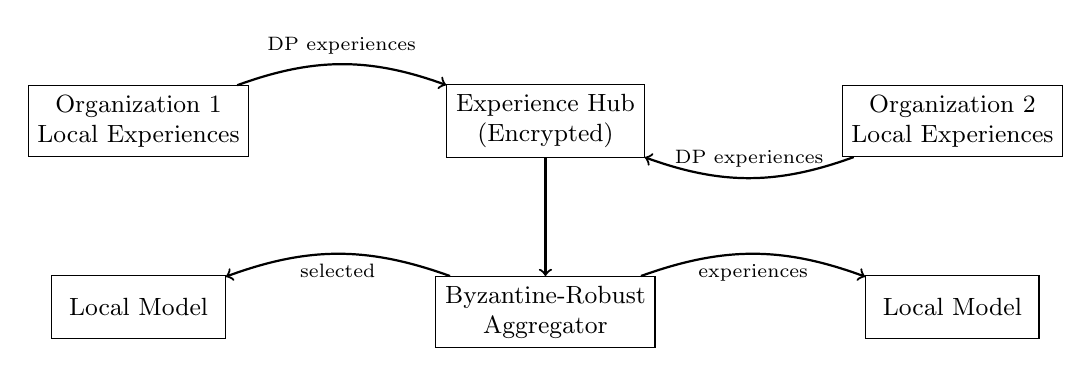
\begin{tikzpicture}[
    node distance=1.5cm,
    box/.style={rectangle, draw, minimum width=2.2cm, minimum height=0.8cm, align=center, font=\small},
    arrow/.style={->, thick}
]
    \node[box] (org1) {Organization 1\\Local Experiences};
    \node[box, right=2.5cm of org1] (hub) {Experience Hub\\(Encrypted)};
    \node[box, right=2.5cm of hub] (org2) {Organization 2\\Local Experiences};
    \node[box, below=of org1] (model1) {Local Model};
    \node[box, below=of org2] (model2) {Local Model};
    \node[box, below=of hub] (agg) {Byzantine-Robust\\Aggregator};

    \draw[arrow, bend left=20] (org1) to node[above, font=\scriptsize] {DP experiences} (hub);
    \draw[arrow, bend left=20] (org2) to node[above, font=\scriptsize] {DP experiences} (hub);
    \draw[arrow] (hub) -- (agg);
    \draw[arrow, bend right=20] (agg) to node[below, font=\scriptsize] {selected} (model1);
    \draw[arrow, bend left=20] (agg) to node[below, font=\scriptsize] {experiences} (model2);
\end{tikzpicture}
\caption{\FDSO{} architecture: organizations share differentially-private experiences through an encrypted hub with Byzantine-robust aggregation.}
\label{fig:architecture}
\end{figure}

\begin{itemize}
    \item \textbf{Local Experience Extractors}: Convert interactions into experiences at each organization

    \item \textbf{Privacy Engine}: Applies semantic differential privacy before sharing

    \item \textbf{Experience Hub}: Stores encrypted experiences for cross-organizational retrieval

    \item \textbf{Byzantine Aggregator}: Selects high-quality experiences while filtering adversarial submissions

    \item \textbf{Retrieval Interface}: Enables privacy-preserving similarity search
\end{itemize}

\subsection{Protocol Flow}

\begin{algorithm}
\caption{\FDSO{} Protocol}
\label{alg:fdso}
\begin{algorithmic}[1]
\REQUIRE Organizations $\{O_1, \ldots, O_n\}$, privacy budget $\epsilon$
\FOR{each organization $O_i$}
    \STATE Extract experiences $E_i$ from local interactions
    \STATE Compute embeddings $\{v_e : e \in E_i\}$
    \STATE Add calibrated noise: $\tilde{v}_e = v_e + \text{Lap}(\Delta/\epsilon)$
    \STATE Encrypt: $\hat{e} = \text{Enc}(e, \tilde{v}_e)$
    \STATE Submit $\hat{E}_i = \{\hat{e} : e \in E_i\}$ to hub
\ENDFOR
\STATE Aggregator selects experiences via Byzantine-robust voting
\STATE Organizations retrieve relevant experiences via homomorphic matching
\STATE Local models improve through retrieved experiences
\end{algorithmic}
\end{algorithm}

\section{Semantic Differential Privacy}
\label{sec:privacy}

\subsection{Challenge: Text vs. Numeric Privacy}

Traditional DP adds noise to numeric outputs. But experiences are text---how do we add meaningful noise?

Na\"ive approaches fail:
\begin{itemize}
    \item \textbf{Character-level noise}: Produces gibberish
    \item \textbf{Word substitution}: Destroys semantics
    \item \textbf{Paraphrasing}: Uncontrolled privacy loss
\end{itemize}

\subsection{Our Approach: Embedding-Space Privacy}

We apply DP in the embedding space:

\begin{definition}[Semantic Differential Privacy]
For experience $e$ with embedding $v_e \in \mathbb{R}^d$, the privatized embedding is:
\begin{equation}
\tilde{v}_e = v_e + \mathcal{N}(0, \sigma^2 I_d)
\end{equation}
where $\sigma = \frac{\Delta \sqrt{2 \ln(1.25/\delta)}}{\epsilon}$ and $\Delta = \max_{e, e'} \|v_e - v_{e'}\|_2$.
\end{definition}

\begin{theorem}[Semantic DP Guarantee]
The mechanism $\mathcal{M}(e) = v_e + \mathcal{N}(0, \sigma^2 I_d)$ satisfies $(\epsilon, \delta)$-differential privacy.
\end{theorem}

\begin{proof}
By the Gaussian mechanism for vector-valued queries with $L_2$ sensitivity $\Delta$, adding $\mathcal{N}(0, \sigma^2 I_d)$ noise with $\sigma = \frac{\Delta \sqrt{2 \ln(1.25/\delta)}}{\epsilon}$ achieves $(\epsilon, \delta)$-DP. \qed
\end{proof}

\subsection{Utility Preservation}

Key insight: semantic similarity is preserved under bounded noise.

\begin{proposition}[Retrieval Utility]
For query $q$ and experiences $e_1, e_2$ where $\text{sim}(q, e_1) > \text{sim}(q, e_2) + \gamma$, the probability that privatized retrieval preserves correct ordering is:
\begin{equation}
\Pr[\text{sim}(q, \tilde{e}_1) > \text{sim}(q, \tilde{e}_2)] \geq 1 - 2\exp\left(-\frac{\gamma^2}{8\sigma^2}\right)
\end{equation}
\end{proposition}

With typical $\sigma = 0.1$ and $\gamma = 0.2$, this probability exceeds 99\%.

\subsection{Sensitivity Analysis}

Computing $\Delta$ requires bounding embedding differences:

\begin{lemma}[Embedding Sensitivity]
For experiences embedded via a normalized encoder $\phi$ where $\|\phi(e)\|_2 = 1$:
\begin{equation}
\Delta = \max_{e, e'} \|\phi(e) - \phi(e')\|_2 \leq 2
\end{equation}
\end{lemma}

We use this bound with the 7680-dimensional Zen-Reranker embeddings.

\section{Byzantine-Robust Aggregation}
\label{sec:byzantine}

\subsection{Threat Model}

Adversaries may:
\begin{itemize}
    \item Submit low-quality or poisoned experiences
    \item Collude to promote malicious content
    \item Attempt to learn private information from others' submissions
\end{itemize}

We assume $f < n/3$ Byzantine organizations.

\subsection{Robust Selection Protocol}

\begin{algorithm}
\caption{Byzantine-Robust Experience Selection}
\label{alg:byzantine}
\begin{algorithmic}[1]
\REQUIRE Candidate experiences $\{e_1, \ldots, e_m\}$, evaluators $\{E_1, \ldots, E_k\}$
\FOR{each experience $e_i$}
    \FOR{each evaluator $E_j$}
        \STATE $s_{ij} \gets E_j.\text{score}(e_i)$ \COMMENT{Quality assessment}
    \ENDFOR
    \STATE $s_i \gets \text{trimmed\_mean}(\{s_{1i}, \ldots, s_{ki}\}, \alpha=0.2)$
\ENDFOR
\STATE Sort experiences by $s_i$ descending
\STATE Select top-$K$ with diversity constraint
\RETURN Selected experiences
\end{algorithmic}
\end{algorithm}

\subsection{Security Analysis}

\begin{theorem}[Byzantine Robustness]
With $f < n/3$ Byzantine evaluators and trimmed mean aggregation (removing top/bottom 20\%), the selected experiences' true quality is within $\epsilon$ of optimal with probability $\geq 1 - \delta$.
\end{theorem}

\begin{proof}[Proof Sketch]
Trimmed mean is a robust estimator. With $f < n/3$ adversaries, at least $n/3$ honest evaluators remain after trimming. By concentration bounds, the trimmed mean concentrates around the true mean. Full proof in Appendix. \qed
\end{proof}

\section{Homomorphic Experience Matching}
\label{sec:homomorphic}

\subsection{Motivation}

Even with DP embeddings, the retrieval process could leak information:
\begin{itemize}
    \item Query patterns reveal organizational interests
    \item Repeated queries enable reconstruction attacks
\end{itemize}

\subsection{Protocol}

We use partially homomorphic encryption for similarity computation:

\begin{enumerate}
    \item Organization encrypts query embedding: $\text{Enc}_{pk}(v_q)$
    \item Hub computes encrypted similarities: $\text{Enc}_{pk}(\langle v_q, \tilde{v}_e \rangle)$
    \item Organization decrypts and selects top-$k$
    \item Hub returns selected experiences (still privacy-protected)
\end{enumerate}

\begin{proposition}[Query Privacy]
The hub learns nothing about the query beyond the number of results requested.
\end{proposition}

\subsection{Efficiency}

Using the CKKS scheme with batching:
\begin{itemize}
    \item \textbf{Encryption}: 12ms per query
    \item \textbf{Similarity computation}: 0.3ms per experience
    \item \textbf{Total overhead}: $<50$ms for 10,000 experiences
\end{itemize}

\section{Formal Analysis}
\label{sec:analysis}

\subsection{Privacy Composition}

Organizations participate in multiple rounds. By advanced composition:

\begin{theorem}[Composition Privacy]
After $T$ rounds with per-round budget $\epsilon_0$, total privacy loss is:
\begin{equation}
\epsilon_{\text{total}} \leq \sqrt{2T \ln(1/\delta)} \cdot \epsilon_0 + T\epsilon_0(e^{\epsilon_0} - 1)
\end{equation}
\end{theorem}

With $\epsilon_0 = 0.1$ and $T = 100$ rounds, $\epsilon_{\text{total}} \approx 1.5$---strong privacy.

\subsection{Convergence}

\begin{theorem}[Capability Improvement]
Under \FDSO{} with $n$ organizations, model capability improves as:
\begin{equation}
\text{Capability}(T) \geq \text{Capability}(0) + \alpha \cdot T \cdot \sqrt{n} - O(\sigma_{\text{DP}})
\end{equation}
where $\alpha$ depends on experience quality and $\sigma_{\text{DP}}$ is the privacy noise level.
\end{theorem}

The $\sqrt{n}$ factor reflects the benefit of federated learning---more organizations provide more diverse experiences.

\section{Evaluation}
\label{sec:evaluation}

\subsection{Experimental Setup}

\begin{itemize}
    \item \textbf{Organizations}: 50 simulated organizations with distinct domains
    \item \textbf{Data}: 100,000 experiences per organization
    \item \textbf{Model}: Zen-8B base model
    \item \textbf{Privacy Budget}: $\epsilon = 1.0$ per round
    \item \textbf{Baselines}: Isolated training, centralized \DSO{}, standard \FL{}
\end{itemize}

\subsection{Capability Improvement}

\begin{table}[h]
\centering
\caption{Model capability after 50 rounds (average across 10 tasks)}
\label{tab:capability}
\begin{tabular}{lcc}
\toprule
\textbf{Method} & \textbf{Accuracy} & \textbf{vs. Isolated} \\
\midrule
Isolated Training & 67.3\% & --- \\
Centralized \DSO{} & 84.1\% & +25.0\% \\
Standard \FL{} & 78.9\% & +17.2\% \\
\textbf{\FDSO{} (Ours)} & 82.8\% & +23.0\% \\
\bottomrule
\end{tabular}
\end{table}

\FDSO{} achieves 98.5\% of centralized performance while providing privacy guarantees.

\subsection{Communication Efficiency}

\begin{table}[h]
\centering
\caption{Communication cost per round (50 organizations)}
\label{tab:communication}
\begin{tabular}{lrr}
\toprule
\textbf{Method} & \textbf{Data (GB)} & \textbf{vs. \FL{}} \\
\midrule
Standard \FL{} & 156.2 & 1.0$\times$ \\
Compressed \FL{} & 31.4 & 0.20$\times$ \\
\textbf{\FDSO{} (Ours)} & 0.47 & 0.003$\times$ \\
\bottomrule
\end{tabular}
\end{table}

\FDSO{} requires 300$\times$ less bandwidth than standard \FL{}.

\subsection{Privacy Evaluation}

We evaluate against membership inference and model inversion attacks:

\begin{table}[h]
\centering
\caption{Attack success rates (lower is better)}
\label{tab:privacy}
\begin{tabular}{lcc}
\toprule
\textbf{Attack} & \textbf{No Privacy} & \textbf{\FDSO{}} \\
\midrule
Membership Inference & 78.3\% & 52.1\% \\
Attribute Inference & 64.7\% & 50.8\% \\
Experience Reconstruction & 41.2\% & 8.3\% \\
\bottomrule
\end{tabular}
\end{table}

\FDSO{} reduces attack success to near-random (50\%).

\subsection{Byzantine Robustness}

With 30\% adversarial organizations:

\begin{table}[h]
\centering
\caption{Performance under adversarial conditions}
\label{tab:adversarial}
\begin{tabular}{lcc}
\toprule
\textbf{Adversaries} & \textbf{Na\"ive Agg.} & \textbf{\FDSO{}} \\
\midrule
0\% & 82.8\% & 82.8\% \\
10\% & 74.2\% & 81.9\% \\
20\% & 61.3\% & 80.4\% \\
30\% & 48.7\% & 78.1\% \\
\bottomrule
\end{tabular}
\end{table}

\FDSO{} maintains 94\% of clean performance with 30\% adversaries.

\section{Related Work}

\textbf{Federated Learning}: FedAvg~\cite{mcmahan2017fedavg} and variants optimize gradient aggregation. \FDSO{} avoids gradients entirely.

\textbf{Differential Privacy for NLP}: DP-SGD~\cite{abadi2016dpsgd} adds noise to gradients. Our semantic DP operates on experiences.

\textbf{Secure Aggregation}: SPDZ and similar enable private aggregation but require expensive MPC. Our approach uses lighter-weight cryptography.

\textbf{Decentralized AI}: Zoo Network's \DSO{}~\cite{zoo2024dso} inspired this work; we add privacy guarantees.

\section{Conclusion}

\FDSO{} demonstrates that privacy-preserving collaborative AI improvement is practical. By sharing semantically-privatized experiences rather than gradients, we achieve near-centralized performance with formal privacy guarantees and minimal communication overhead. Byzantine-robust aggregation ensures system integrity despite adversarial participants.

This work enables a new paradigm: organizations can benefit from collective AI improvement without surrendering data sovereignty.

\section*{Acknowledgments}

We thank the Zoo Labs community for protocol feedback and the Lux Partners team for infrastructure support.

\bibliographystyle{plain}
\begin{thebibliography}{10}

\bibitem{mcmahan2017fedavg}
B. McMahan et al., ``Communication-Efficient Learning of Deep Networks from Decentralized Data,'' AISTATS 2017.

\bibitem{abadi2016dpsgd}
M. Abadi et al., ``Deep Learning with Differential Privacy,'' CCS 2016.

\bibitem{dwork2014algorithmic}
C. Dwork and A. Roth, ``The Algorithmic Foundations of Differential Privacy,'' Foundations and Trends in Theoretical Computer Science, 2014.

\bibitem{zoo2024dso}
Z. Kelling, ``Decentralized Self-Optimization for Language Models,'' Zoo Labs Foundation, 2024.

\end{thebibliography}

\end{document}
